\documentclass[11pt]{article}

\usepackage{fancyhdr}
\usepackage[letterpaper]{geometry}
\usepackage[latin2]{inputenc}
\usepackage{graphicx}
\usepackage{ulem}
\usepackage{amsmath}

\pagestyle{fancyplain}
\lhead{\large{CSE 015: Discrete Mathematics}}
\rhead{\large{Fall Semester 2017}}


\title{\bf Homework Assignment 4}
\date{Sunday, October 15 2017}
\author{ Pedro Damian Sanchez Jr}

\begin{document}

\maketitle

\begin{figure}
\begin{center}
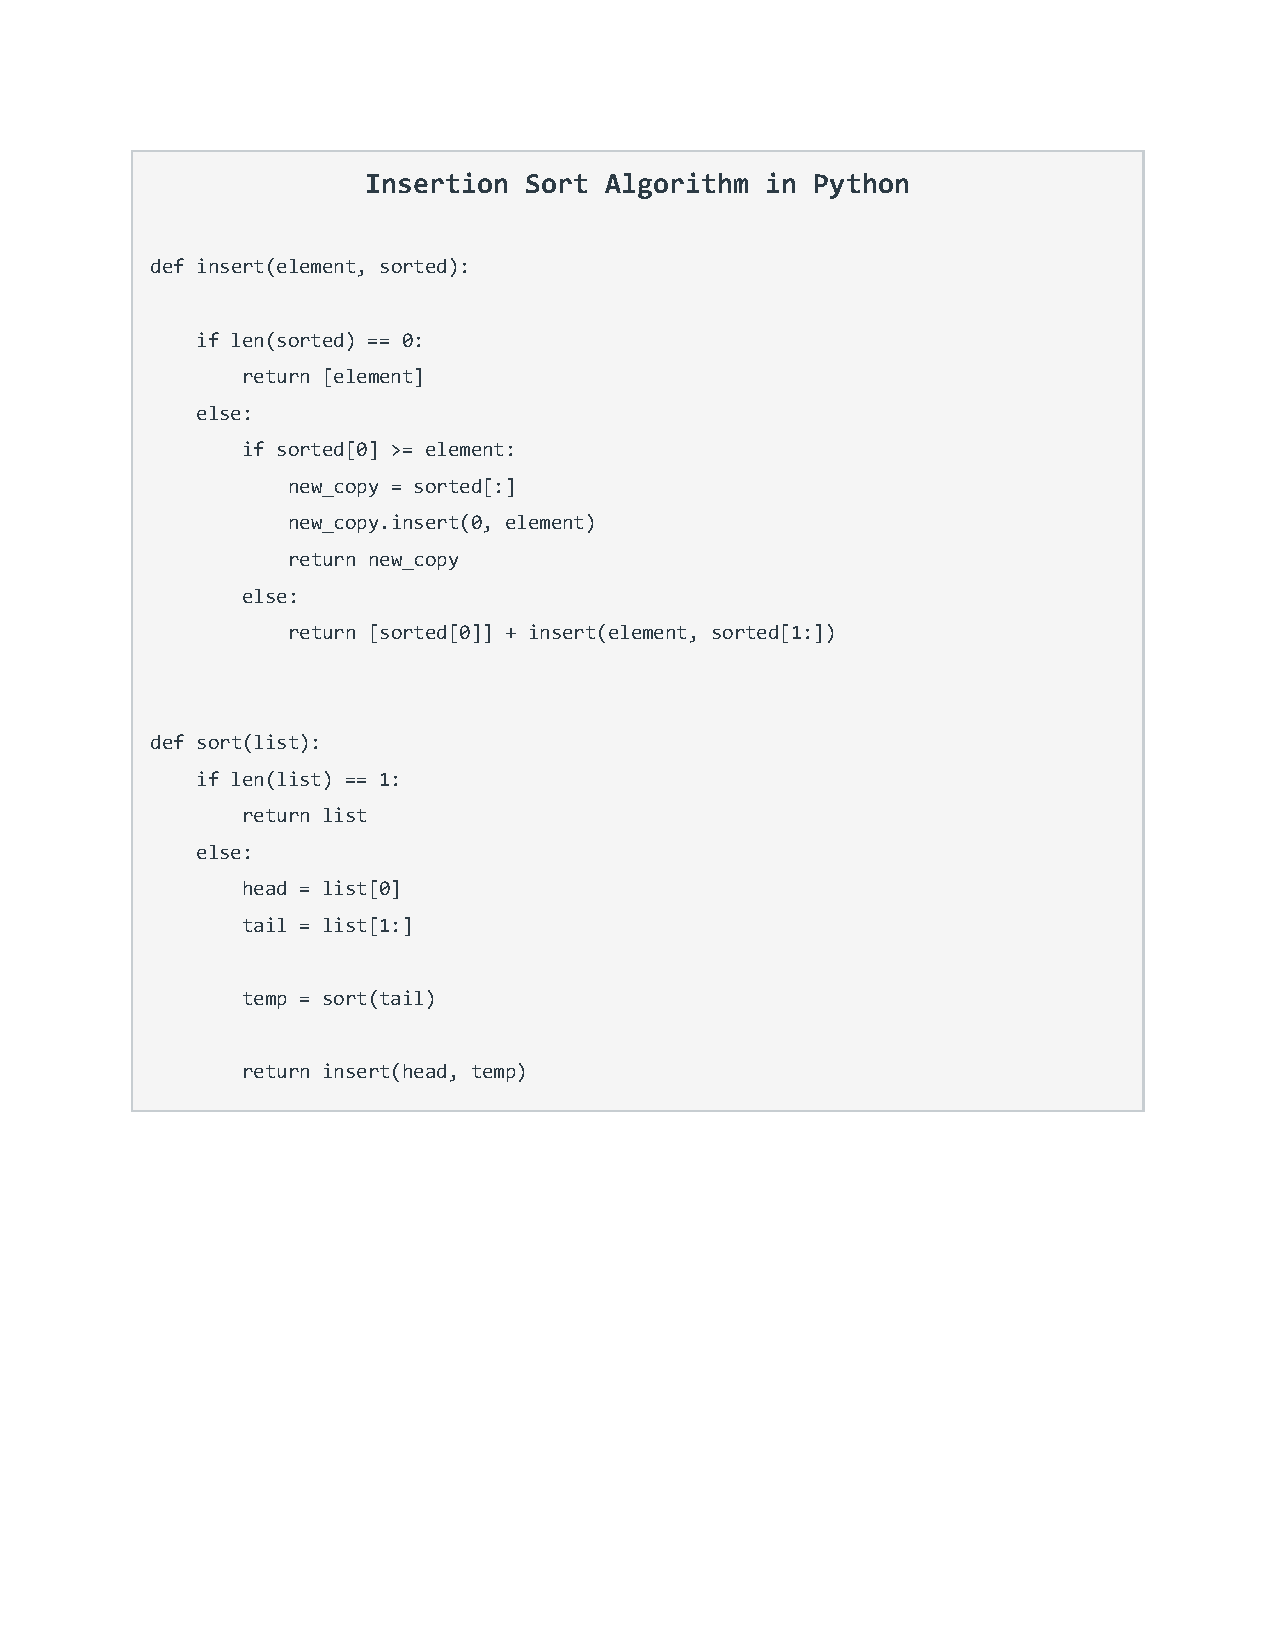
\includegraphics[scale = 0.5]{code.pdf}
\end{center}
\end{figure}

\section{Question 1}

The insert function exhibits what is known as best case / worst case behavior. That is to say that with some inputs, the function will do more comparisons that it would with other inputs. Provide a list of 5 numbers, and another number that has to be inserted into the list, that will force the insert function to perform in its best case (that is as few comparisons as possible). Now provide a list of 5 numbers that will force the insert function to perform in the worst case (as many comparisons as possible).

\section{Question 1 Solution}

A Dynamic Array Stack would prove to be the ideal choice when doing a specific model push. This will double the array size if there is not enough space to perform an insertion into an already sorted list of elements. Copying an array is not possible in real time; therefore, a push operation nesscary to allow the random item insertion to take place.

\begin{table}[h]
\centering
\begin{tabular}{|l|l|l|l|}
\hline
\textbf{Push()} & \textbf{copy} & \textbf{old array size} & 
\textbf{new array size} \\
\hline
\textbf{1} & \textbf{0} & \textbf{1} & \textbf{-} \\
\hline
\textbf{2} & \textbf{1} & \textbf{1} & \textbf{2} \\
\hline
\textbf{3} & \textbf{2} & \textbf{2} & \textbf{4} \\
\hline
\textbf{4} & \textbf{0} & \textbf{4} & \textbf{-} \\
\hline
\textbf{5} & \textbf{4} & \textbf{4} & \textbf{8} \\
\hline
\end{tabular}
\end{table}

Note how 3 pushes will require $2 + 1 = 3$ copies, 5 pushes will require $4 + 2 + 1 = 7$ copies, and, 9 pushes will require $8 + 4 + 2 + 1 = 15$ copies. \\
\\
It can be said that in a general case, $2^{n}+1$ number of pushes will require $2^n+ 2^{n-1} + ... + 2 + 1 = 2^{n+1} - 1$ copies to perform a sort.\\ 

\section{Question 2}

What is the order of complexity of the insert function in the worst case? You are required to provide a complexity function, and a proof that your complexity function belongs to a particular complexity class. In your complexity function you may specify the number of comparisons performed, as a function of input size.

\section{Question 2 Solution}

In the best case where the sorted list is empty, inserting a new element occurs in $\bf O(1)$ length of time. If the new element being inserted is less than or equal to the first element in the sorted list, then inserting the new element into first position occurs in the order of $\bf O(1)$. However, if the new element is greater than first element of the list, then, calling the insert function for appending first element of the list will automatically repeat the operation. Therefore, in this worst case we have to call the insertion function for all elements in the list when the new element is greater than every other element in the list, making the operation run in $\bf O(n)$ length of time.

\section{Question 3}

What is the order of complexity of the overall sort procedure?

\section{Question 3 Solution}

It then becomes apparent, that, the sorting algorithm discussed above occurs in the order of $\bf O(n)$, and, every each call of the sorting algorithm also occurs in the order of $\bf O(n)$. \\
\\
Hence, the overall order of complexity of the Insertion Sort Function is $\bf O(n^2)$. \\



\end{document}
